Bei einer Achterbahn fährt der Wagenzug unten in einen vertikalen Looping vom Radius \rLpO. Der Winkel $\alpha$ gibt die Lage des Wagenzugs an, vom tiefsten Punkt aus gemessen.

\begin{center}
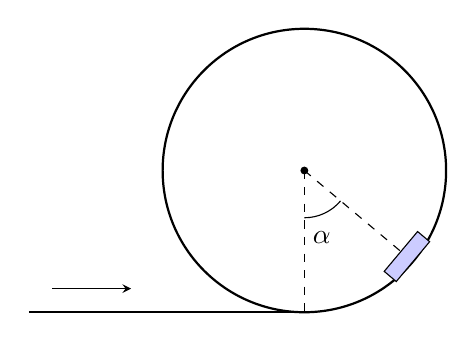
\begin{tikzpicture}[>=stealth]
 \draw[thick] (0,0) circle (1.8);
 \draw[thick] (-3.5,-1.8) -- (0,-1.8);
 \fill (0,0) circle (0.05);
 \draw[dashed] (0,0) -- (0,-1.8);
 \draw[dashed] (0,0) -- (1.379,-1.157);
 \draw (0,-0.6) arc (-90:-40:0.6);
 \node at (0.22,-0.85) {$\alpha$};
 \fill[blue!20] (1.167,-1.410) -- (1.591,-0.904) -- (1.438,-0.775) -- (1.014,-1.281) -- cycle;
 \draw (1.167,-1.410) -- (1.591,-0.904) -- (1.438,-0.775) -- (1.014,-1.281) -- cycle;
 \draw[->] (-3.2,-1.5) -- (-2.2,-1.5);
\end{tikzpicture}
\end{center}

\begin{abcliste}
\abc Zeichnen Sie in einer Skizze die für die Zentripetalkraft auf den Wagenzug verantwortlichen Kräfte für die Winkel $\alpha = 0$ (tiefster Punkt), $\pi/2$, $3\pi/4$ und $\pi$ (höchster Punkt) ein. Achten Sie darauf, dass die Kräfte im richtigen Verhältnis zueinander stehen.
\abc Wie schnell muss der Wagenzug im höchsten Punkt mindestens fahren?
\end{abcliste}
